\documentclass[tikz,border=10pt]{standalone}
\usepackage{tikz}
\usetikzlibrary{shapes,arrows,positioning,calc,fit,backgrounds,decorations.pathreplacing,arrows.meta,patterns}

\begin{document}
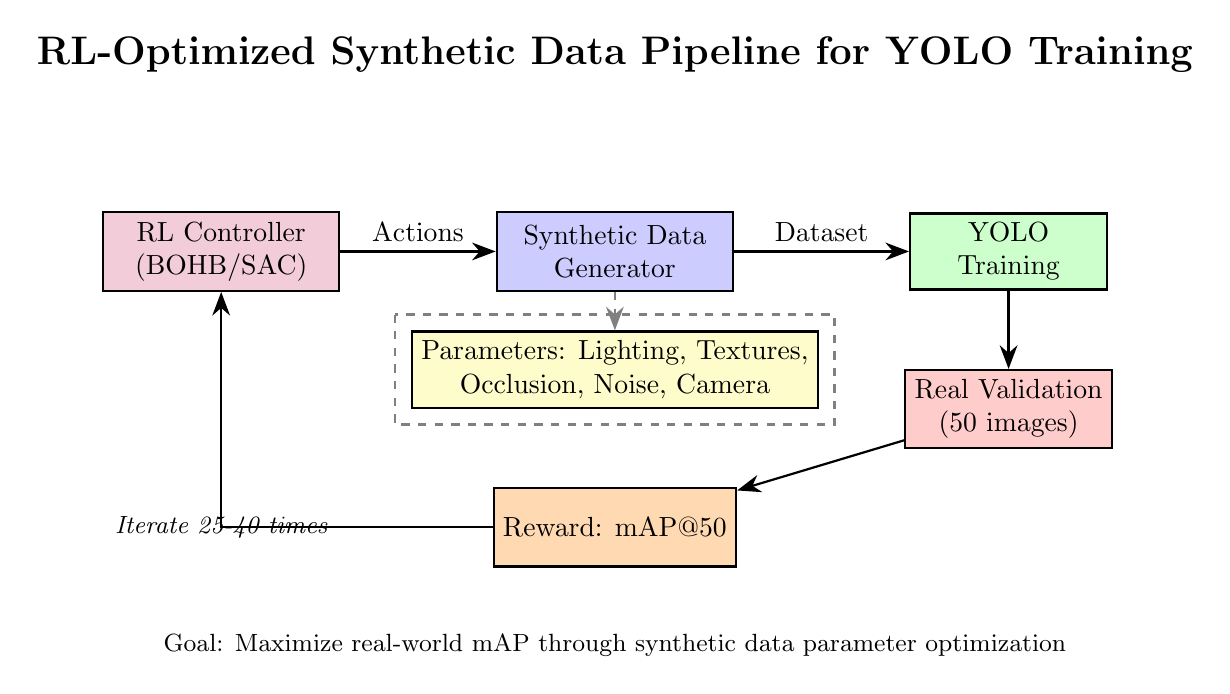
\begin{tikzpicture}[
    node distance=1.5cm,
    box/.style={rectangle, draw=black, thick, minimum width=3cm, minimum height=1cm, align=center, fill=blue!10},
    process/.style={rectangle, draw=black, thick, minimum width=2.5cm, minimum height=0.8cm, align=center, fill=green!10},
    data/.style={rectangle, draw=black, thick, minimum width=2.5cm, minimum height=0.8cm, align=center, fill=orange!10},
    arrow/.style={-{Stealth[length=3mm]}, thick}
]

% Title
\node[font=\Large\bfseries] at (5, 5) {RL-Optimized Synthetic Data Pipeline for YOLO Training};

% RL Controller
\node[box, fill=purple!20] (rl) at (0, 2.5) {RL Controller\\(BOHB/SAC)};

% Synthetic Data Generator
\node[box, fill=blue!20] (synth) at (5, 2.5) {Synthetic Data\\Generator};

% Parameter space annotation
\node[data, fill=yellow!20, minimum width=4cm] (params) at (5, 1) {Parameters: Lighting, Textures,\\Occlusion, Noise, Camera};

% YOLO Training
\node[process, fill=green!20] (yolo) at (10, 2.5) {YOLO\\Training};

% Real Validation
\node[data, fill=red!20] (real) at (10, 0.5) {Real Validation\\(50 images)};

% mAP Reward
\node[box, fill=orange!30] (reward) at (5, -1) {Reward: mAP@50};

% Arrows
\draw[arrow] (rl) -- node[above] {Actions} (synth);
\draw[arrow] (synth) -- node[above] {Dataset} (yolo);
\draw[arrow] (yolo) -- (real);
\draw[arrow] (real) -- (reward);
\draw[arrow] (reward) -| (rl);

% Dashed box around parameter space
\draw[dashed, thick, gray] (params.north west) +(-0.2, 0.2) rectangle ($(params.south east) + (0.2, -0.2)$);
\draw[arrow, dashed, gray] (synth) -- (params);

% Iteration label
\node[font=\small\itshape] at (0, -1) {Iterate 25-40 times};

% Legend
\node[font=\small] at (5, -2.5) {Goal: Maximize real-world mAP through synthetic data parameter optimization};

\end{tikzpicture}
\end{document}
